%!TEX root=qsic2014.tex
% mainfile: qsic2014.tex

\begin{figure*}[!t]
\centering
\captionsetup{justification=centering}
  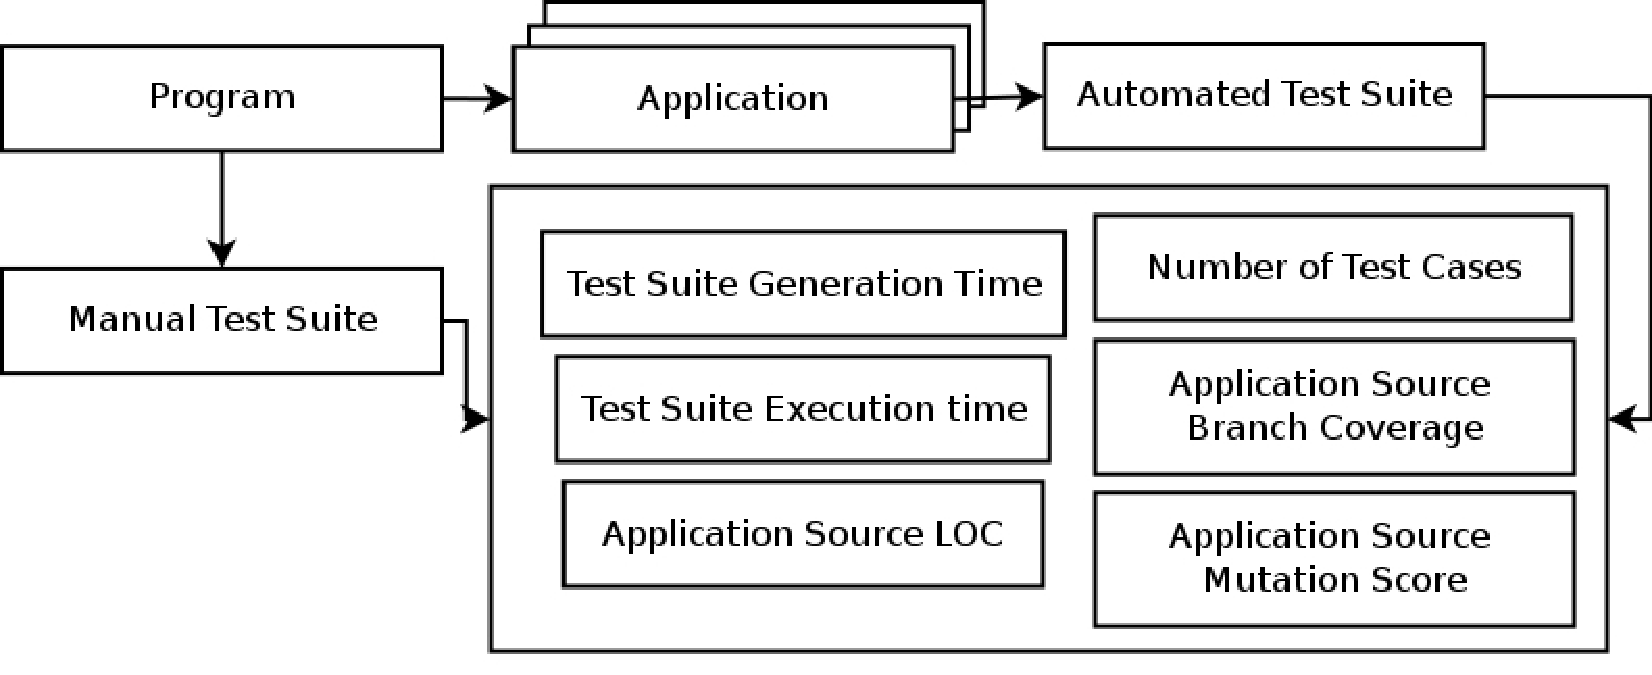
\includegraphics[width=\linewidth]{proccess_diagram.pdf}
    \caption{Evaluation Process}
  \label{fig:process_diagram}
\end{figure*}
%KJ: MAKE NEW DIAGRAM!!

\section{Empirical Evaluation}
\label{sec:evaluation}
Given the many different techniques for generating test suites, the primary goal of this paper's empirical study is to compare the quality and complexity of the resulting test suites.  We implemented the empirical evaluation approach as shown in Figure~\ref{fig:process_diagram}.  As can be seen in the figure, existing programs are fed into automatic test suite generators to create executable test suites.  These test suites are then compared to the programs' associated, manually written test suites based on \textcolor{red}{SOME NUMBER} metrics.   

The goals of the experiments are as follows:
\squishlist
\item stuff1
\item stuff2
\item stuff3
\item stuff 4
\squishend

\subsection{Experiment Design and Metrics}
All experiments were performed on GNU/Linux workstations with kernel 3.2.0-44, a 2 GHz Intel Corporation Xeon E5/Core i7 processor and  15.6 GB of main memory. 
Ten programs were identified from the SF110 code suite~\cite{fraser:2012}.  The case study applications were selected due to their size, the existence of associated manually developed JUnit test cases, and their use in tuning EvoSuite parameters for mutation and test generation, one of our test suite generation tools.  Table~\ref{tbl:program_table} provides a list of the selected SF110 programs with their respective lines of code (LOC) and average cyclomatic complexity per method.  LOC and Cyclomatic complexity were measured using JavaNCSS~\cite{leejavancss}.  

Netweaver is the largest program under consideration with nearly 18K lines of code.  Netweaver has an average Cyclomatic Complexity ($CC$) of 2.82 across all methods, which implies that for a specific method $M$, 1) $CC_M$ is an upper bound for the number of test cases that are necessary to achieve a complete branch coverage within the method $M$, and 2) $CC_M$ is a lower bound for the number of paths through the control flow graph. Assuming each test case takes one path, the number of cases needed to achieve path coverage is equal to the number of paths that can actually be taken, ignoring infeasible paths.  The smallest, Jni-inchi has around 800 lines of code with an average cyclomatic complexity of 2.05.  

\begin{table}[!t]
\caption{Benchmark Programs and their Properties}
\label{tbl:program_table}
\resizebox{\columnwidth}{!}{%
\begin{tabular}{|l|c|c|}
\hline
\textbf{Program} & \textbf{LOC} &\textbf{Cyclomatic Complexity} \\ \hline
Netweaver                              & 17953                              & 2.82                                                \\ \hline
Inspirento                             & 1769                               & 1.76                                                \\ \hline
Jsecurity                              & 9470                               & 2.05                                                \\ \hline
Saxpath                                & 1441                               & 2.10                                                \\ \hline
Jni-inchi                              & 783                                & 2.05                                                \\ \hline
Xisemele                               & 1399                               & 1.29                                                \\ \hline
Diebierse                              & 1539                               & 1.74                                                \\ \hline
Lagoon                                 & 6060                               & 3.52                                                \\ \hline
Lavalamp                               & 1039                               & 1.50                                                \\ \hline
Jnfe                                   & 1294                               & 1.38                                                \\ \hline
\end{tabular}
}
\end{table}

After the case study applications were identified and analyzed, automated test tools EvoSuite and Codepro were used to generate test suites. As EvoSuite is non-deterministic, ten sets of tests were generated for evaluation.  

\subsubsection{Evaluation Metrics}
We then took the manual and automated generated test suites and used several different tools to
collect the metrics. MAJOR is used find the mutation score of the program, JaCoCo is used to attain the branch coverage,
and JavaNCSS measures the lines of code and the cyclic complexity of the programs. Time to create the tests was also
recorded manually to compare Evosuite and CodePro. Time to create the manual tests was available with the SF110.

Because Evosuite uses a genetic algorithm to generate unit tests, we generated the tests for Evosuite ten times for each program. With multiple datasets, we can more accurate results with the standard deviation between mutation score, coverage, and time. CodePro uses a deterministic algorithm to generate the tests, so multiple test suite generations were not needed. With results gathered from Evosuite, CodePro, and the manually written tests, we then compared the scores based upon complexity, time to generate test suite, mutation score, lines of code, and branch coverage.

\subsection{Experiments and Results}

\subsection{Threats to Validity}
